\section{Background and contributions}
\Gls{ibc} systems refer to a class of data-intensive feedback control systems whose feedback is provided by camera sensor(s) (see Fig.~\ref{fig:ch6_IBC_block_diagram}). 
 The combination of camera sensor(s) and image processing algorithms is capable of detecting a rich set of features in an image that can be used to compute the states of the system such as relative position or distance, depth perception, and tracking of the object-of-interest~\cite{pendleton2017perception}. 
 The challenge, however, is that there is an inherent long sensing delay due to compute-intensive image processing algorithms~\cite{saidi2018future}.  

A typical implementation of an \gls{ibc} system uses an optimal \gls{lqr}~\cite{dorf2011modern} considering the worst-case image workload and thus has worst-case sensing delay~\cite{saidi2018future} (illustrated in Fig.~\ref{fig:ch6_workload_IBC}).
However, this results in poor effective resource utilisation in a multiprocessor platform, and suboptimal \gls{qoc}~\cite{fontantelli2013optimal}. 
Multiprocessor platforms with high processing power that allow parallel and pipelined executions can be used to cope with this long worst-case sensing delay. 
The sensing algorithms may be parallelised (whenever possible, but limited by the degree of application parallelism) if the algorithmic structure is known (white/grey box) and thus reduce the worst-case sensing delay \cite{saidi2018future}. 
Pipelined control implementation executes the sensing algorithm in a pipelined fashion 
with the worst-case sensing delay and thus reduces the effective actuation and sampling rate~\cite{medina2019designing},~\cite{krautgartner1998performance}.
The advantage of a pipelined implementation is that it is applicable even if the application algorithm is a black box.
Note that for nominal control implementation, the sensor-to-actuator delay $\tau$ is at most equal to the sampling period $h$, whereas for a pipelined control implementation $\tau$ is greater than $h$.

However, pipelining is limited by inter-frame dependencies, i.e., the data or algorithmic dependencies between consecutive frame processing, e.g., due to video coding~\cite{li2015lagrangian} or visual tracking~\cite{smeulders2013visual}. 
Inter-frame dependence time (denoted by $\fd$) can be quantified for the current image frame as the maximum time required to complete the processing of (parts of) the algorithm the subsequent image frame processing depends on. 
Alternatively, $\fd$ is the maximum time required to wait between processing consecutive image frames. 

\begin{figure}[t]
    \centerline{
     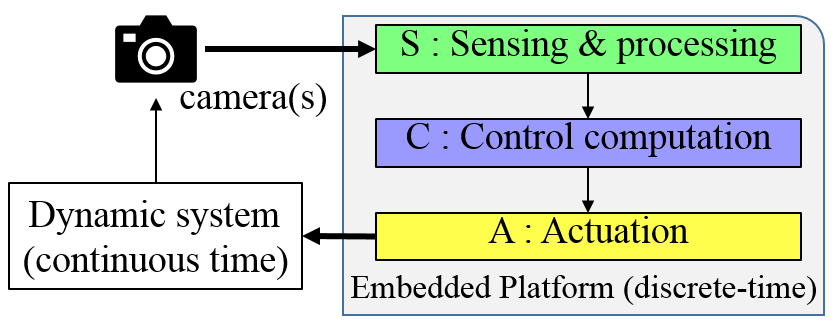
\includegraphics[width=0.6\textwidth]{images/IBC_bd2.png}
    }
    %\vspace{-1em}
    \caption{An \gls{ibc} system: block diagram (repeating Fig.~\ref{fig:ch1_ibc_intro}~(a), for readability)}
    \label{fig:ch6_IBC_block_diagram}
     \vspace{-2em}
\end{figure}

The sensing delay due to the compute-intensive processing (sensing) of the image stream is dependent on image workload variations, which occur due to image content and result in a wide range between best-case and worst-case image-processing times.
It is known from \cite{fontantelli2013optimal} that explicitly taking into account workload variations in controller design improves the \gls{qoc}.
Workload variations are typically considered as a variable delay or stochastic delay in standard sampled-data linear control design techniques~\cite{ogata1995discrete}.

In current literature, workload variations are typically considered only for sequential \gls{ibc} implementation~\cite{fontantelli2013optimal} and not for pipelined implementation~\cite{medina2019designing},~\cite{krautgartner1998performance} (see Fig.~\ref{fig:ch6_pipelined_IBC}). 
In~\cite{medina2019implementation}, pipelining is considered along with variable delay but the inter-frame dependencies are neglected.
Further, these approaches do not consider system nonlinearities, i.e., the variations in system dynamics, and constraints imposed on the system variables, which can be crucial when considering a practical implementation. 
E.g., the maximum steering angle of the Udacity self-driving car is set to +/- 25 degree~\cite{tian2018deeptest} and the vehicle velocity is kept constant for the simulations in~\cite{kosecka1997vision}.  

The main motivation of this work is to address limitations of the state-of-the-art pipelined multiprocessor \gls{ibc} approaches that do not take into account inter-frame dependencies, system constraints and nonlinearities for the application of interest.
These limitations make it difficult for these approaches to be realised in real systems. 

\textbf{Contribution:} We extend the basic \gls{spade} flow (introduced in Chapter \ref{chap:parallelisation}) for \gls{ibc} system design for pipelined implementation without parallelising the sensing task. Our approach explicitly takes into account the inter-frame dependencies. Further, we present an adaptive predictive control formulation based on \gls{lpv} \gls{io} models for a pipelined multiprocessor implementation of \gls{ibc} systems while considering workload variations, system nonlinearities and constraints on system variables, and thus makes a step forward towards real-life adoption.
We also compare the proposed formulation with the state-of-the-art multiprocessor \gls{ibc} system implementations.

\begin{figure}
\centerline{
    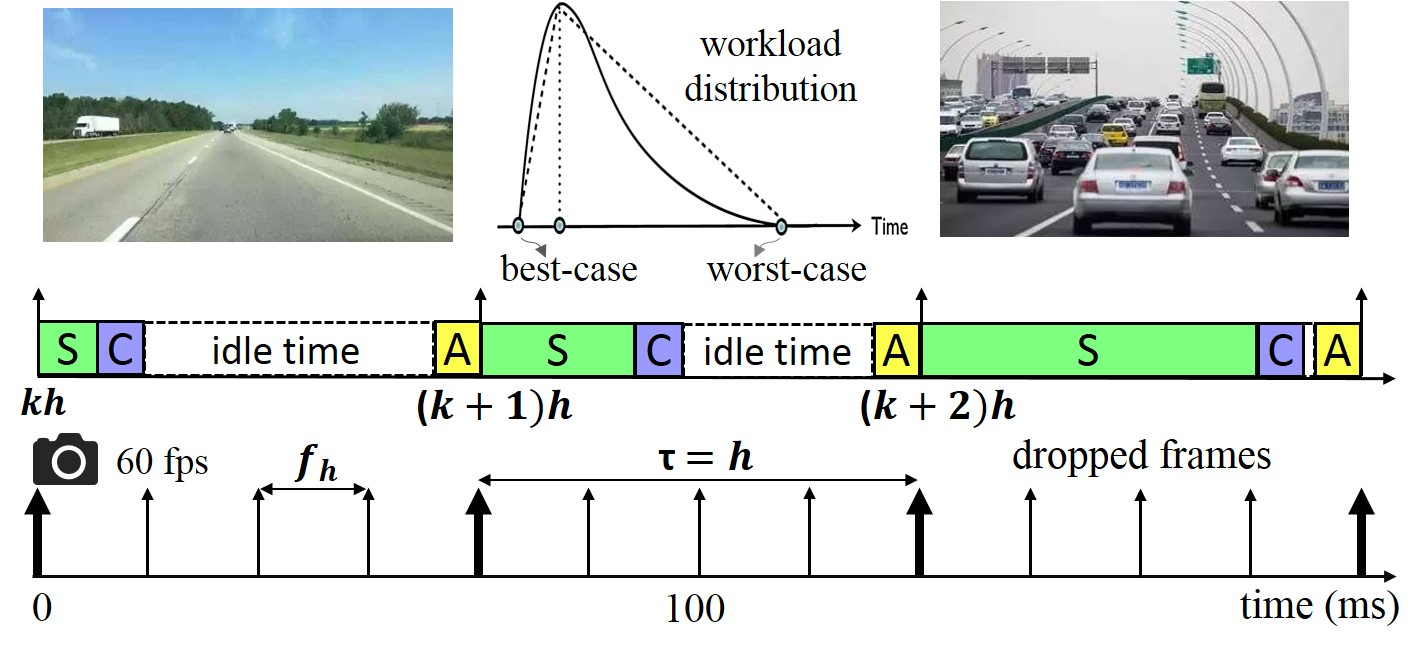
\includegraphics[width=\textwidth]{images/ibc_workload.jpg}
    }
    \caption{Illustration of a workload distribution and a sequential \gls{ibc} implementation considering worst-case image workload. (Adapted from Fig.~\ref{fig:ch1_ibc_intro}~(b) and (c), for readability).
    }
    \label{fig:ch6_workload_IBC}
    \vspace{-2em}
\end{figure}

Recent advances in numerical optimization for \gls{mpc} have enabled safety-critical applications on embedded platforms, such as engine control and powertrain coordination in the automotive domain~\cite{GMODYS2018engine,GMODYS2018powertrain}. 
Moreover, the latest methods such as those recently reported in~\cite{sparseNMPC} suggest that the model and \gls{mpc} tuning parameters can be adapted at runtime without reconstructing the optimization problem. 
This allows implementing adaptive \gls{mpc} with the same computational complexity as the non-adaptive case.
An \gls{mpc} formulation is thus advantageous for use in image-based control systems where, due to constraints, nonlinearities and workload variations, an adaptive control method that maximizes control performance is desirable.